\documentclass[10pt, conference]{IEEEtran}
\usepackage[english]{babel}
\usepackage[usenames]{color}
\usepackage{colortbl}
\usepackage{comment}
\usepackage{graphicx}
\usepackage{epsfig}
\usepackage{array, colortbl}
\usepackage{listings}
\usepackage{epstopdf}
\usepackage{multirow}
\usepackage{rotating}
%\usepackage{subfigure}
%\usepackage{subfig}
\usepackage{float}
\usepackage[obeyspaces,hyphens,spaces]{url}
\usepackage{balance}
\usepackage{fancybox}
\usepackage{scalefnt}
\usepackage[normalem]{ulem}
%\pagestyle{plain}
\pagenumbering{arabic}
\pagestyle{empty}
\clubpenalty = 10000
\widowpenalty = 10000
\displaywidowpenalty = 10000
\usepackage{cleveref}

\usepackage{graphicx}
\usepackage{caption}
\usepackage{subcaption}


\makeatletter
\renewcommand{\paragraph}[1]{\noindent\textsf{#1}.}

\title{Our Title}
\author{Mika V. M\"antyl\"a$^{1}$, Foutse Khomh$^{2}$, Bram Adams$^{2}$, Emelie Engstr\"om$^{3}$, Kai Petersen$^{4}$
    \\
    \emph{$^{1}$ Dep. of Computer Science and Engineering, Aalto University, Finland}
    \\
    \emph{$^{2}$ SWAT--MCIS, \'{E}cole Polytechnique de Montr\'{e}al, Qu\'{e}bec, Canada}
    \\
    \emph{$^{3}$ Dep. of Computer Science, Lund University, Sweden}
    \\
    \emph{$^{4}$ School of Computing, Blekinge Institute of Technology, Sweden}
    \\
    \emph{mika.mantyla@aalto.fi, \{foutse.khomh, bram.adams\}@polymtl.ca, emelie.engstr\"om@cs.lth.se, kai.petersen@bth.se }}

\begin{document}
\maketitle

\begin{abstract}
One of the most important challenges to migrate software application to Cloud is to choose the right instance type, which gives the right resources to our application. Our analysis based upon five benchmarks on five Cloud instances provides a difference of performance, helping users to choose the right instance for their applications. 
\end{abstract}

\section{Introduction}
\label{sec:introduction}

Quisque a dignissim purus. Vivamus ut ultrices orci, ac tincidunt magna. Mauris lacinia feugiat dignissim. Donec congue mi risus, in cursus eros adipiscing eu. Proin cursus nulla et sapien vulputate feugiat. Mauris vehicula consectetur ipsum non lobortis. Nunc nec eros fermentum, suscipit purus nec, sagittis metus. Sed vulputate nisl in dapibus condimentum. Aliquam erat volutpat. Proin vitae aliquet ante. Maecenas vulputate nisl ac tellus volutpat, vel pulvinar risus tincidunt. In hac habitasse platea dictumst. Etiam tincidunt sit amet turpis aliquet tristique.

\section{Background and Related Work}
\label{sec:backgr-relat-work}

\subsection{Instances}

\begin{table*}
\begin{center}
\begin{tabular}{|l|l|l|l|l|l|}
  \hline
  Instance type & \# virtual CPU & Memory (GiB) & Instance storage & EBS-Optimized Available & Network performance \\
  \hline
  t2.micro & 1 & 1 & EBS Only & No & Low to moderate \\
  t2.small & 1 & 2 & EBS Only & No & Low to moderate \\
  t2.medium & 2 & 4 & EBS Only & No & Low to moderate \\
  c3.large & 2 & 3.75 & 2 x 16 (SSD) & No & Moderate \\
  c3.xlarge & 4 & 7.5 & 2 x 40 (SSD) & Yes & Moderate \\
   \hline
\end{tabular}
\caption{\label{table:instances} Characteristics of each instance of our case study}
\end{center}
\end{table*}


We have used in our case study five different instances based on Ubuntu. The Table \ref{table:instances} provides their differences 





\subsection{Benchmarks}

In this section, we provide the Benchmarks used in our analyzes. We have used \textit{UnixBench} to analyze the CPU performance, \textit{dd if=/dev/zero of=sb-io-test bs=1M count=1k conv=fdatasync} to analyze the IO, ioping to analyze IOPS, Redis to analyze the memory performance, and Dbench to analyze Disk and Network Throughput performances. 

\subsubsection{UnixBench}


UnixBench is a benchmark used to evaluate the general performances of a server, specially it is used to measure the CPU. It runs the following tests:

\begin{itemize}

\item Dhrystone: This test focus on the operations on the strings.
\item Whetstone: This test focus on the operations on the floats.
\item Execl Throughput: This test aims at measuring the number of call \textit{execl} that could be done by second.
\item Pipe Throughput: This test aims at evaluating the pipes' bandwidth, a process read or write on a pipe.
\item Pipe-based Context Switching: This test aims at measuring the communication between process.
\item Process Creation: 
\item Shell Scripts: It represents the execution time of a script by simulating the common operations. 
\item System Call Overhead: 

\end{itemize}

\subsubsection{dd if=/dev/zero of=sb-io-test bs=1M count=1k conv=fdatasync}

This benchmark is used to compute the performance of reading/writing on a disc, bellow this command : \textit{dd if=/dev/zero of=sb-io-test bs=1M count=1k conv=fdatasync}. The command \textit{dd} is used to copy a file by the selection of just a part of the file. The parameters of this command are:

\begin{itemize}

\item if: What we should write, in our example, we write NULL (/dev/zero).
\item of: The file name where the command \textit{dd} writes.
\item bs: The size of block to write.
\item count: The count of blocks to write. 
\item conv: The conversion to do. For example: \textit{conv=lcase} will convert the character to lower case characters.

\end{itemize}

Therefore, the command \textit{dd if=/dev/zero of=sb-io-test bs=1M count=1k conv=fdatasync} is used to evaluate the performance of Disk IO. It will copy in the file \textit{sb-io-tests}, 1M x 1k NULL (/dev/zero).

It gives as results, the record-in, record-out, the size copied, the time spent to copy data, and the copy speed.

\subsubsection{ioping}

By the same principle of the command \textit{ping}, which evaluate the network latency, we have the command \textit{ioping} used to measure the monitor I/O latency. However, it does many request, we can limit the number of request by the parameter \textit{-c number\_of\_requests}. It gives as results the minimum, the average, the maximum time of all requests done.

\subsubsection{Redis}

\indent Redis is an open source, in-memory advanced key-value store with optional persistence to disk. Redis command line interface ${redis-cli}$ is used to analyze the Redis metrics and access the actual data. Redis includes the redis-benchmark utility which is used to evaluate the performance of memory using simulates running commands done by $N$ clients at the same time sending $M$ total queries. Basic syntax of redis benchmark is shown below:\\

\indent redis-benchmark [option] [option value]\\

\indent When Redis-benchmark is run, lots of tet with specific definitions are done as following:

\begin{itemize}

\item PING-INLINE and PING-BULK: This command is often used to test if a connection is still alive, or to measure latency.
\item SET: It Set key to hold the string value. If key already holds a value, it is overwritten, regardless of its type. Any previous time to live associated with the key is discarded on successful SET operation.
\item GET: It Get the value of key. If the key does not exist the special value nil is returned. An error is returned if the value stored at key is not a string, because GET only handles string values.
\item INCR: This comment increments the number stored at key by one. If the key does not exist, it is set to 0 before performing the operation. An error is returned if the key contains a value of the wrong type or contains a string that can not be represented as integer. This operation is limited to 64 bit signed integers.
\item LPUSH: This comment insert all the specified values at the head of the list stored at key. If key does not exist, it is created as empty list before performing the push operations. When key holds a value that is not a list, an error is returned.
It is possible to push multiple elements using a single command call just specifying multiple arguments at the end of the command. Elements are inserted one after the other to the head of the list, from the leftmost element to the rightmost element.
\item LPOP: It removes and returns the first element of the list stored at key.
\item SADD: Add the specified members to the set stored at key. Specified members that are already a member of this set are ignored. If key does not exist, a new set is created before adding the specified members. An error is returned when the value stored at key is not a set.
\item SPOP:This command removes and returns a random element from the set value stored at key.
\item LRANGE: Returns the specified elements of the list stored at key. The offsets start and stop are zero-based indexes, with 0 being the first element of the list (the head of the list), 1 being the next element and so on. These offsets can also be negative numbers indicating offsets starting at the end of the list. For example, -1 is the last element of the list, -2 the penultimate, and so on. Note that if you have a list of numbers from 0 to 100, LRANGE list 0 10 will return 11 elements, that is, the rightmost item is included.
\item MSET:  MSET replaces existing values with new values, just as regular SET. See MSETNX if you don't want to overwrite existing values. MSET is atomic, so all given keys are set at once. It is not possible for clients to see that some of the keys were updated while others are unchanged.
\end{itemize}

\subsubsection{Dbench}
\indent Dbench is a Filesystem benchmark which generates load patterns, but without requiring a lab of Windows load generators to run. It is used to calculate the performance of Disk and Network Troughput. Dbench is a utility to benchmark a system based on client workload profiles.\\
\indent Dbench takes only one parameter on the command line, which is the number of processes (clients) to start. Issuing the command “dbench 30” for example, creates 30 parallel processes of dbench. All processes are started at the same time and each of them runs the same workload. The workload for each dbench process is specified by a client.txt configuration file in the working (testing) directory. It consists of a mixture of file system operations executed by each dbench process. dbench runs with n parallel processes and delivers only one value as a result. The resulting value is an average throughput of the file system operations described in client.txt and measured in megabytes per second.\\
\indent It can also take the following options:\\

\begin{itemize}
\item -c client.txt : Use this as the full path name of the client.txt file (the default is $/usr/share/dbench/client.txt$).
\item -s: Use synchronous file IO on all file operations.
\item -t TIME: set the runtime of the benchmark in seconds (default 600)
\item -D DIR: set the base directory to run the filesystem operations in
\item -x: enable xattr support, simulating the xattr operations Samba4 would need to perform to run the load
\item -S: Use synchronous IO for all directory operations (unlink, rmdir, mkdir and rename). The tbench program takes a number, which indicates the number of clients to run simultaneously,  and a server name: $tbench_srv$ should be invoked on that server before invoking tbench. tbench can also take the following options:
\item -c loadfile: Use this as the full path name of the client.txt file (the default is $/usr/share/dbench/client.txt$).
\item -T option[,...]: This sets the socket options for the connection to the server. 
\end{itemize}


\section{Approach}
\label{sec:approach}

In this section, we provide the approach used to extract data. While the first step consists of creating the instances, the second one consists of computing data. 

We have created the first instance of type \textit{t2.micro}, we have also created a script to compute data. Therefore, to create another instance, we have used the image of the first one. Hence, we have created the types of instances consisting of \textit{t2.small}, \textit{t2.medium}, \textit{c3.large}, and \textit{c3.xlarge}.

To compute data, we have used the benchmarks described above. Since the performance of Cloud instances change over time, because there are many instances deployed in the same hardware, we execute each one five times.

We have extracted data in csv form, as described in the Figure .... .  

\section{Results}
\label{sec:results}

In this section, we provide the benchmarks results.

\subsection{CPU performances}

\textbf{Results. The averages of UnixBensh results for each instance are: 1952.12 for the instance \textit{t2.micro}, 1800.18 for the instance \textit{t2.small}, 2660.04 for the instance \textit{t2.medium}, 2269.7 for the instance \textit{c3.large}, and 3273.46 for the instance \textit{c3.xlarge}}.

\begin{figure}
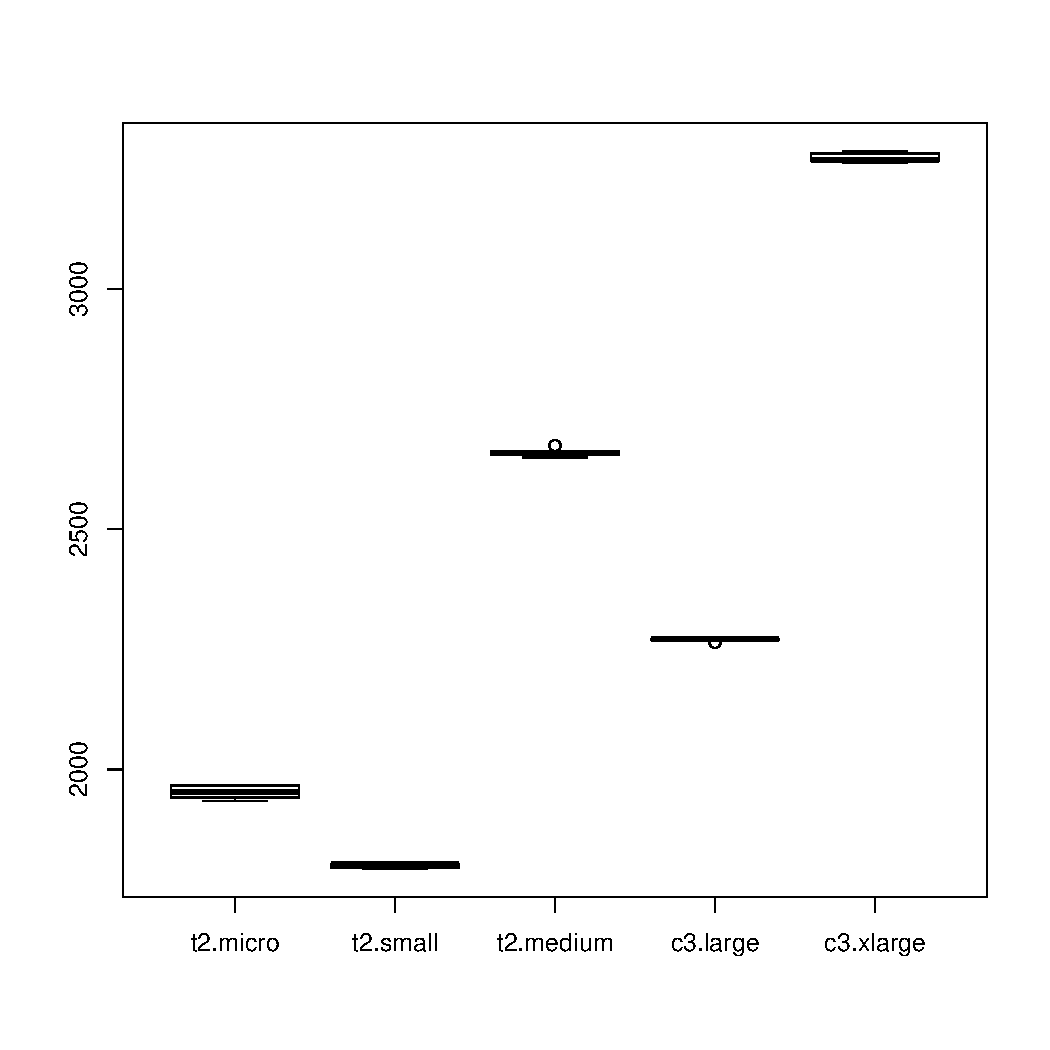
\includegraphics[width=0.5\textwidth]{plots/UnixBench.pdf}
\caption{UnixBench results}
\label{fig:UnixBenchResult}
\end{figure}

As highlighted by Figure \ref{fig:UnixBenchResult}. The minimum value of \textit{UnixBench} benchmark results for the instance \textit{t2.micro} is \textit{1933.5}, whereas the maximum is \textit{1967}. The minimum for the instance \textit{t2.small} is \textit{1793.6} and the maximum is \textit{1806.8}. \textit{t2.medium} provides as a minimum result of the same benchmark \textit{2649.2}, where the maximum is \textit{2674.1}. The minimum value of \textit{c3.large} is \textit{2264.2} where the maximum is \textit{2271.8}. \textit{c3.xlarge} provides a minimum of \textit{3263.1} and a maximum of \textit{c3.xlarge}.

The smallest value of \textit{UnixBench} benchmark is provided by the instance \textit{t2.small}, and the maximum is provided by the instance \textit{c3.xlarge}.

As provided by Figure \ref{fig:UnixBenchResult}, the order of instances by the \textit{UnixBench} benchmark is as follow: \textit{t2.small, t2.micro, c3.large, t2.medium, c3.xlarge}.

\textbf{Discussion}. We observe that we have three categories of instances in Figure \ref{fig:UnixBenchResult}. We can classify the instances in three main clusters. While the first one is represented by the instances \textit{t2.micro} and \textit{t2.small}, which have one virtual processor. The second category is presented by \textit{t2.medium} and \textit{c3.large}, which contains two virtual processor. The third category contains the instance \textit{c3.xlarge}, it contains 4 virtual CPU. Hence, the difference between the three category is due to the number of virtual processor.

Moreover, There is a difference between the instances \textit{t2.micro} and \textit{t2.small}. By analyzing the benchmark results, we have found that the main difference is in the test \textit{File Copy 4096 bufsize 8000 maxblocks}, which consists of copying a large size, which gives the important different score (around 5910.3 for the instance \textit{t2.micro} and 4998.4 for the instance \textit{t2.small}). 

The difference between \textit{t2.medium} and \textit{c3.large} is principally due to the test \textit{Dhrystone 2 using register variables}. It tests the operations on the strings. In this test, \textit{t2.medium} has a score of 5449.3, whereas \textit{c3.large} has a score of 3408.7.

\subsection{IO performances}

\begin{figure}
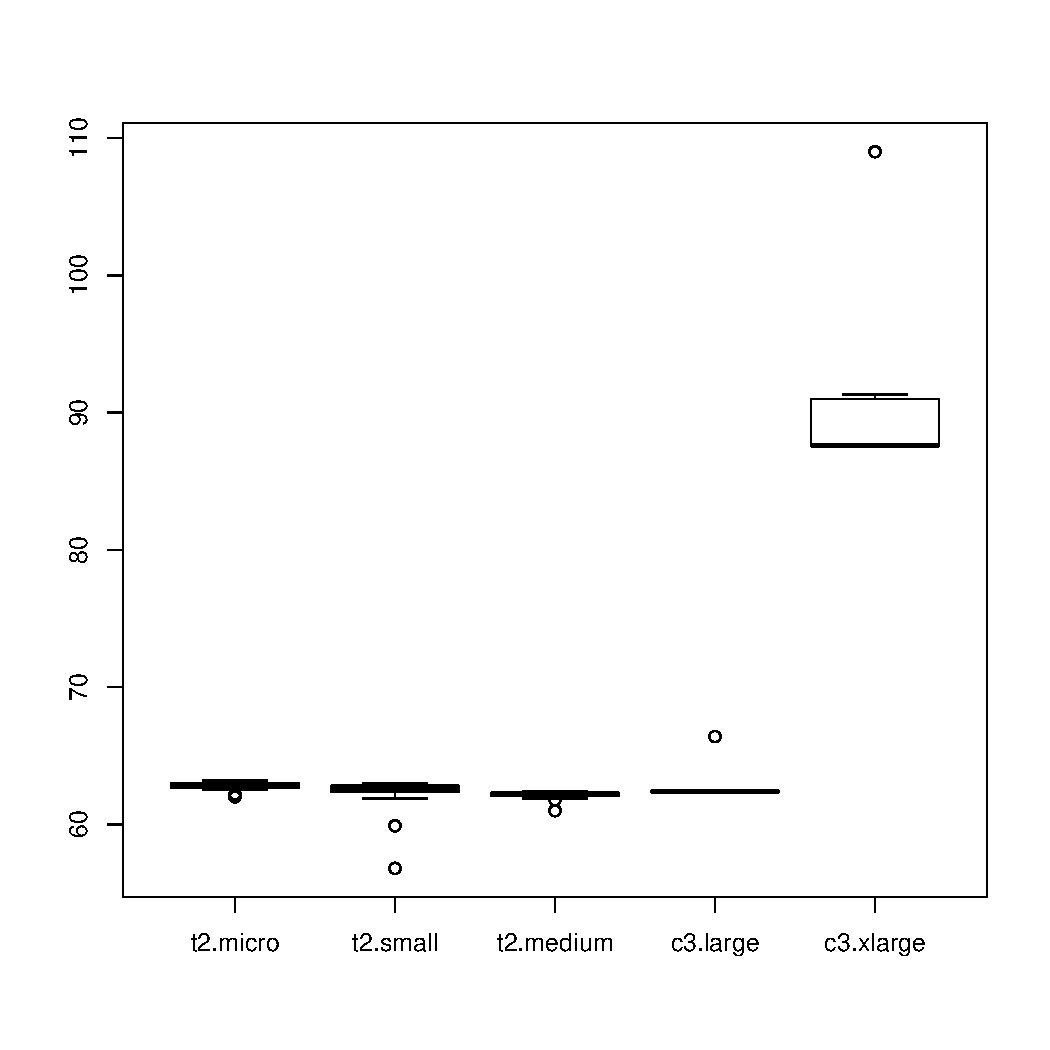
\includegraphics[width=0.5\textwidth]{plots/dd.pdf}
\caption{IO benchmark results}
\label{fig:ddResult}
\end{figure}

\textbf{Results. The averages of IO Benchmark results for each instance are: 62.68 for the instance \textit{t2.micro}, 62.7 for the instance \textit{t2.small}, 61.98 for the instance \textit{t2.medium}, 63.2 for the instance \textit{c3.large}, and 91.88 for the instance \textit{c3.xlarge}}

As highlighted by Figure \ref{fig:ddResult}. The minimum value of \textit{IO} benchmark results for the instance \textit{t2.micro} is \textit{62.1 MB/s}, whereas the maximum is \textit{63.1 MB/s}. The minimum for the instance \textit{t2.small} is \textit{62.5 MB/s} and the maximum is \textit{62.8 MB/s}. \textit{t2.medium} provides as a minimum result of the same benchmark \textit{61.8 MB/s}, where the maximum is \textit{62.3 MB/s}. The minimum value of \textit{c3.large} is \textit{62.4 MB/s} where the maximum is \textit{66.4 MB/s}. \textit{c3.xlarge} provides a minimum of \textit{87.6 MB/s} and a maximum of \textit{109 MB/s}.

The smallest value of \textit{IO} benchmark is provided by the instance \textit{t2.medium}, and the maximum is provided by the instance \textit{c3.xlarge}.

As provided by Figure \ref{fig:ddResult}, the order of instances by the \textit{IO} benchmark is as follow: \textit{ t2.medium, c3.large, t2.small, t2.micro, c3.xlarge}.


\textbf{Discussion.} From the comparison provided in Figure \ref{fig:ddResult}, the instance \textit{c3.xlarge} has the highest speed of reading/Writing on disk. We refer these results to the I/O Performances, where the instance \textit{c3.xlarge} has "Moderate/500Mbps", and the other instances have "Low to moderate" or "Moderate".

\subsection{IOPS performances}


\begin{figure*}
	\begin{subfigure}[b]{0.24\textwidth}
                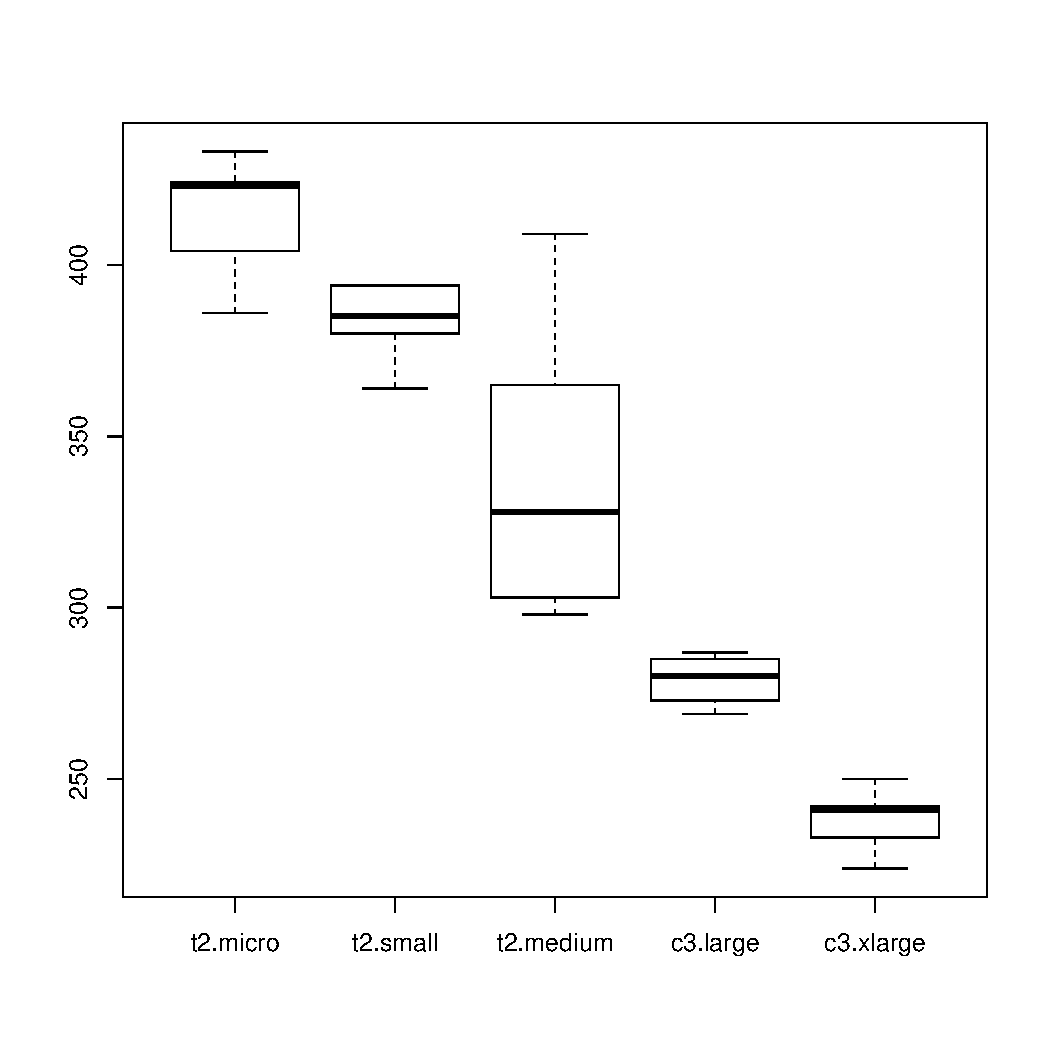
\includegraphics[width=\textwidth]{plots/iopingMin.pdf}
                \caption{Min}
                \label{fig:min}
        \end{subfigure}
        \begin{subfigure}[b]{0.24\textwidth}
                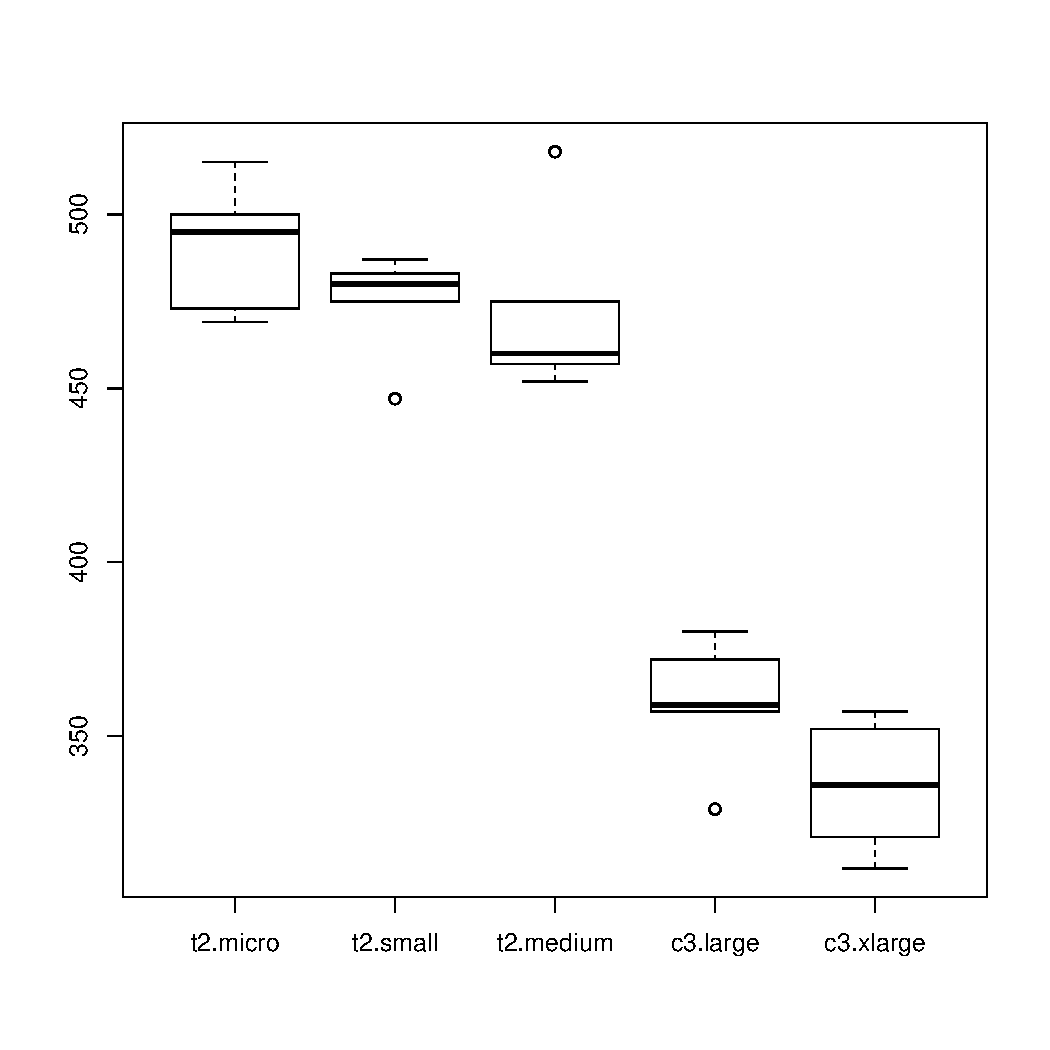
\includegraphics[width=\textwidth]{plots/iopingAvr.pdf}
                \caption{Average}
                \label{fig:avr}
        \end{subfigure}
        \begin{subfigure}[b]{0.24\textwidth}
                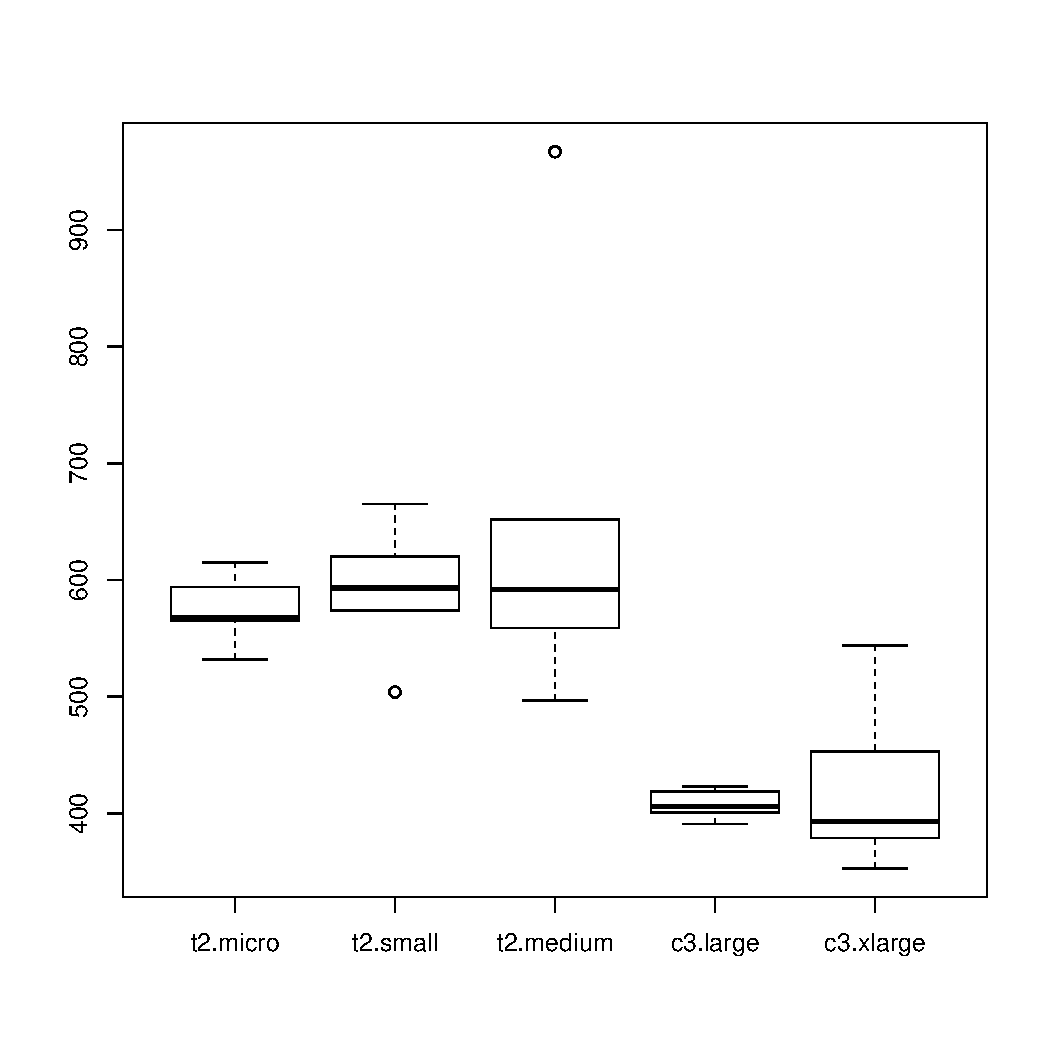
\includegraphics[width=\textwidth]{plots/iopingMax.pdf}
                \caption{Max}
                \label{fig:max}
        \end{subfigure}
         \begin{subfigure}[b]{0.24\textwidth}
                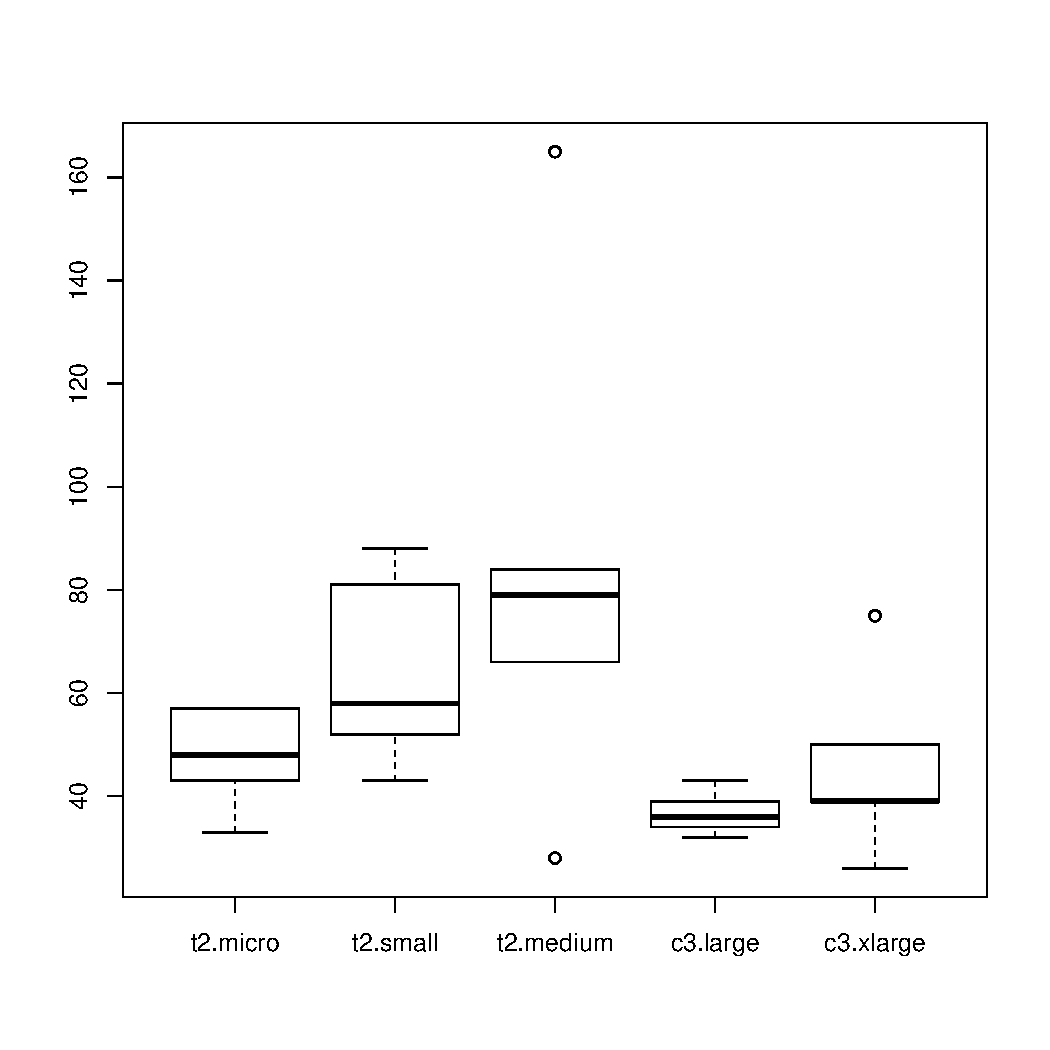
\includegraphics[width=\textwidth]{plots/iopingMdev.pdf}
                \caption{MDev}
                \label{fig:mdev}
        \end{subfigure}
        \caption{\label{fig:IOPSResults} IOPS benchmark comparison of results (us)}
\end{figure*}

\begin{center}
\begin{table}
\begin{center}
\begin{tabular}{|l|l|l|l|l|}
  \hline
t2.micro & t2.small & t2.medium & c3.large & c3.xlarge \\
\hline
386 us	& 385 us & 409 us & 285 us & 242 us \\
424 us & 394 us & 365 us & 273 us & 241 us \\
423 us & 	364 us & 303 us & 287 us & 233 us \\
404 us & 	394 us & 328 us & 269 us & 224 us \\
433 us & 	380 us & 298 us & 280 us & 250 us \\
\hline
\end{tabular}
\caption{\label{IOPSResultsMin} IOPS min results}
\end{center}
\end{table}
\end{center}

\begin{center}
\begin{table}
\begin{center}
\begin{tabular}{|l|l|l|l|l|}
  \hline
t2.micro & t2.small & 	t2.medium & 	c3.large & 	c3.xlarge \\
\hline 
469 & 	480 & 	457 & 	372 & 	336 \\
473 & 	447 & 	475 & 	329 & 	352 \\
515 & 	487 & 	452 & 	359 & 	357 \\
495 & 	475 & 	518 & 	380 & 	321 \\
500 & 	483 & 	460 & 	357 & 	312 \\
\hline
\end{tabular}
\caption{\label{IOPSResultsAvr} IOPS average results}
\end{center}
\end{table}
\end{center}


\begin{center}
\begin{table}
\begin{center}
\begin{tabular}{|l|l|l|l|l|}
  \hline
t2.micro & t2.small & 	t2.medium & 	c3.large & 	c3.xlarge \\
\hline 
568	& 	620	& 	497	& 	419	& 393 \\
532	& 	504	& 	652	& 	391	& 	453 \\
594	& 	665	& 	559	& 	406	& 	544 \\
615	& 	593	& 	967	& 	423	& 	379 \\
565	& 	574	& 	592	& 	401	& 	353 \\
\hline
\end{tabular}
\caption{\label{IOPSResultsMax} IOPS Max results}
\end{center}
\end{table}
\end{center}


\begin{center}
\begin{table}
\begin{center}
\begin{tabular}{|l|l|l|l|l|}
  \hline
t2.micro & t2.small & 	t2.medium & 	c3.large & 	c3.xlarge \\
\hline 
57 &	81 &	28 &	36 &	39 \\
33 &	43 &	84 &	32 &	50 \\
43 &	88 &	66 &	39 &	75 \\
57 &	58 &	165 &	43 &	39 \\
48 &	52 &	79 &	34 &	26 \\
\hline
\end{tabular}
\caption{\label{IOPSResultsMDev} IOPS MDev results}
\end{center}
\end{table}
\end{center}

\textbf{Table \ref{IOPSResultsMin}, Table \ref{IOPSResultsAvr}, Table \ref{IOPSResultsMax}, and Table \ref{IOPSResultsMDev} provide the results of the benchmark used to evalute the IOPS performance}. While we have used the benchmark ioping to evaluate the performance of IOPS of each instance, the benchmark gives four different results, the first one corresponds to minimum time in the results of one execution, which highlighted in \ref{IOPSResultsMin}. The second one corresponds to the average, provided by Table \ref{IOPSResultsAvr}. The third one represents the maximum time shown by Table \ref{IOPSResultsMax}. Whereas, the third one presented by Table \ref{IOPSResultsMDev} is MDev.

As provided in Figure \ref{fig:min}, each instance has its own minimum time to provide an IOPS result, the instances are ordered as follow: \textit{c3.xlarge, c3.large, t2.medium, t2.small, and t2.micro}.

As provided in Figure \ref{fig:avr}, each instance has its own average time to provide an IOPS result, the instances are ordered as follow: \textit{c3.xlarge, c3.large, t2.medium, t2.small, and t2.micro}.

As provided in Figure \ref{fig:max}, each instance has its own maximum time to provide an IOPS result, the instances are ordered as follow: \textit{c3.xlarge, c3.large, t2.micro, t2.small, and t2.medium}. \textit{t2.micro, t2.small, and t2.medium} have approximately the same value as a mediam. 

As provided in Figure \ref{fig:mdev}, each instance has its own MDev value, the instances are ordered as follow: \textit{c3.xlarge, c3.large, t2.micro, t2.small, and t2.medium}.

\subsection{Disk performances}


\begin{center}
\begin{table}
\begin{center}
\begin{tabular}{|l|l|l|l|l|}
  \hline
t2.micro & t2.small & 	t2.medium & 	c3.large & 	c3.xlarge \\
\hline 
196.735 &	232.123 &	255.073 &	287.458 & 354.273 \\
196.843 &	231.064 &	259.235 &	287.348 &	350.399 \\
197.842 &	232.38 &	256.889 &	287.161 &	353.942 \\
197.558 &	230.762 &	255.986 &	286.702 &	353.547 \\
196.474 &	231.347 &	255.956 &	46.8487 &	355.52 \\
\hline
\end{tabular}
\caption{\label{table:DBench2Results} DBench benchmark results (MB/sec)}
\end{center}
\end{table}
\end{center}

\textbf{The averages of DBench results for each instance are: 197.0904 MB/sec for the instance \textit{t2.micro}, 231.5352 MB/sec for the instance \textit{t2.small}, 256.6278 MB/sec for the instance \textit{t2.medium}, 239.10354 MB/sec for the instance \textit{c3.large}, and 353.5362 MB/sec for the instance \textit{c3.xlarge}}. The results are provided in Table \ref{table:DBench2Results}


\begin{figure}
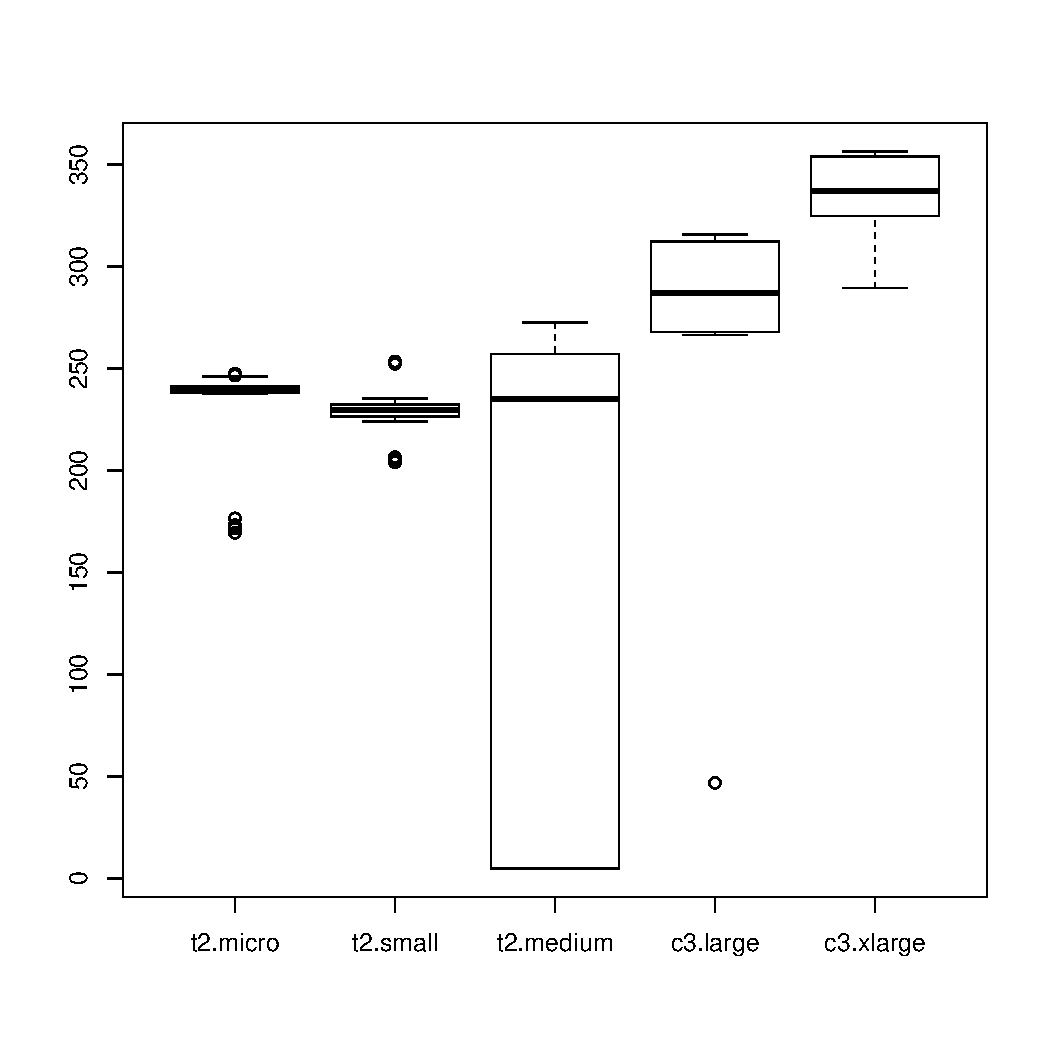
\includegraphics[width=0.5\textwidth]{plots/dbench2.pdf}
\caption{Difference between instances in Disk performances}
\label{fig:dbench2}
\end{figure}

As provided by Figure \ref{fig:dbench2}, the order of instances by the disk performance is as follow: \textit{t2.micro, t2.small, t2.medium, c3.large, and c3.xlarge}.

\textbf{Discussion.} The main differences between the instances \textit{t2.micro} and \textit{t2.small} are the tests \textit{Find}, which consists of finding a file in the disk. Where the second important difference we have found is the test \textit{ReadX} related to the read file operations. Moreover, the important difference between \textit{t2.small} and \textit{t2.medium} is \textit{Flush} test, which is a test related to the file operations. The same difference between \textit{t2.medium} and \textit{c3.large}. The main differences between \textit{c3.xlarge} and \textit{c3.large} are \textit{ReadX} and \textit{WriteX}, which are related to read/write on a file.

\subsection{Network Throughput performances}




\begin{center}
\begin{table}
\begin{center}
\begin{tabular}{|l|l|l|l|l|}
  \hline
t2.micro & t2.small & 	t2.medium & 	c3.large & 	c3.xlarge \\
\hline 
4.63978 &	368.66 &	377.072 &	455.738 &	709.535 \\
4.86367 &	236.93 &	268.571 &	294.85 &	337.944 \\
4.86856 &	238.627 &	266.551 &	295.228 &	342.986 \\
4.9142 &	239.147 &	269.105 &	298.469 &	327.806 \\
4.88602 &	234.173 &	264.574 &	300.31 &	20.7406 \\
\hline
\end{tabular}
\caption{\label{table:DBench10Results} DBench benchmark results (MB/sec)}
\end{center}
\end{table}
\end{center}


\textbf{The averages of DBench results for each instance are: 4.834446 for the instance \textit{t2.micro}, 263.5074 for the instance \textit{t2.small}, 289.1746 for the instance \textit{t2.medium}, 328.919 for the instance \textit{c3.large}, and 347.80232 for the instance \textit{c3.xlarge}}. The results are provided in Table \ref{table:DBench10Results}


\begin{figure}
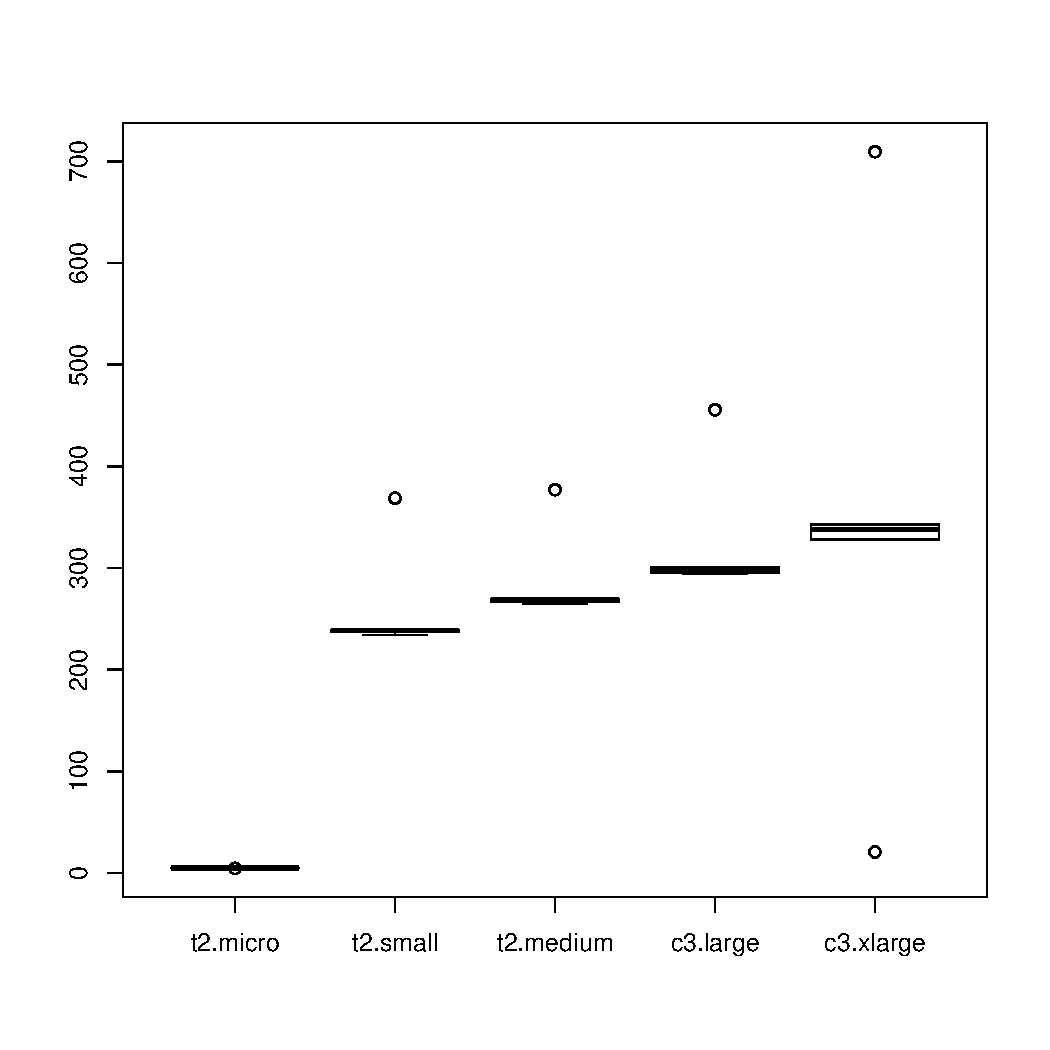
\includegraphics[width=0.5\textwidth]{plots/Dbench10.pdf}
\caption{Difference between instances in Disk performances}
\label{fig:dbench10}
\end{figure}

As provided by Figure \ref{fig:dbench10}, the order of instances by the disk performance is as follow: \textit{t2.micro, t2.small, t2.medium, c3.large, and c3.xlarge}.


\section{Discussion}
\label{sec:discussion}




\section{Comparison of Results}
\label{sec:comparison-results}

\section{Conclusion}
\label{sec:conclusion}

\section*{Acknowledgment}
TODO

\balance
\bibliographystyle{IEEEtran}
\bibliography{assignment.bib}
\end{document}
